%\documentclass[Proof]{elex}
\documentclass{elex}

\usepackage[dvips]{graphicx}
\usepackage{psfrag}

\vol{*}
\no{*}

\title{Homotopy method with a formal stop criterion applied to circuit simulation}

\author{H\'ector V\'azquez-Leal,$^{1a)}$ Luis Hern\'andez-Mart\'{\i}nez,$^{2}$ Arturo Sarmiento-Reyes,$^{2}$ Roberto Casta\~neda-Sheissa,$^{1}$ and Agust{\'i}n Gallardo-Del-\'Angel$^{1}$}

\affiliate{
$^{1}$ School of Electronic Instrumentation and Atmospheric Sciences, University of Veracruz\\
Cto. Gonzalo Aguirre Beltr\'an S/N, Xalapa, Veracruz, M\'exico \\
%
$^{2}$ National Institute for Astrophysics, Optics and Electronics\\
Luis Enrique Error \#1, Sta. Mar\'ia Tonantzintla, Puebla, M\'exico
}

\email{a) hvazquez@uv.mx}

\received{2003}{7}{00}
\accepted{2003}{7}{00}


\setcounter{page}{1}

\begin{document}

\maketitle 

\begin{abstract}
The continuous scaling for fabrication technologies of electronic circuits demands the design of new and improved simulation techniques for integrated circuits. Therefore,
this work shows a new double bounded homotopy based on a polynomial formulation with four lines separated by a fixed distance. The new homotopy scheme presents a bounding between the two internal solution lines and the symmetry axis, which allows to establish a stop criterion for the simulation in CD. Besides, the initial and final points on this new double bounded homotopy can be set arbitrarily. Mathematical properties for the new homotopy will be introduced and exemplified using a benchmark circuit.
\end{abstract}

\begin{keywords}
Homotopy continuation methods, multistable circuits.
\end{keywords}

\begin{classification}
Integrated circuits.
\end{classification}


\begin{thebibliography}{99}
\bibitem{Schwa_book} A. F. Schwarz, {\it Computer-aided design of microelectronic circuits and systems: Volume 1}, Academic Press Inc., 1987).
\bibitem{NEWTONR} C. T. Kelley, ``Solving Nonlinear Equations with Newton's Method,'' {\it SIAM, Fundamentals of Algorithms}, 2003.
\bibitem{green} X. Shou,  L.B. Goldgeisser, and  M.M Green , ``A methodology for constructing two-transistor multistable circuits," International Symposium on Circuits and Systems, Sydney, Australia, pp. 377 - 380, May, 2001.
\bibitem{homo_green2} M. M. Green, ``An efficient continuation method for use in globally convergent dc circuit simulation," 1995 ISSSE Proceedings, San Francisco, USA, pp. 497 - 500, October, 1995.
\bibitem{homo_ArtificialP} R. C. Melville and L. Trajkovic, ``Artificial parameter homotopy methods for the dc operating point problem," {\it IEEE transactions on computer-aided design of integrated circuits and systems} vol. 12, no. 6, pp. 861 - 877, 1997.
\bibitem{BHLHOM} Roychowdhury and R. J. Melville, ``Delivering global dc convergence for large mixed-signal circuits via homotopy/continuation methods," {\it IEEE Transactions on Computer-Aided Design of Integrated Circuits and Systems} vol. 25, no. 1, pp. 66-78, January, 2006.
\bibitem{homo_DWolfMulti} D. M. Wolf and S. R. Sanders, ``Multiparameter homotopy methods for finding dc operating points of nonlinear circuits," {\it IEEE transactions on circuits and systems-I: fundamental theory and aplications} vol. 43, no. 10, pp. 824 - 837, October, 1996.
\bibitem{homo_iscas05} H. V\'azquez-L., L. Hern\'andez-M., and A. Sarmiento-R., ``Double-Bounded Homotopy for analysing nonlinear resistive circuits," International Symposium on Circuits and Systems, Kobe, Japan, pp. 3203 - 3206, May, 2005.
\bibitem{homo_hk05} H. V\'azquez-L., L. Hern\'andez-M., A. Sarmiento-R., and R. Castaneda-S., ``Numerical continuation scheme for tracing the double bounded homotopy for analysing nonlinear circuits," 2005 International Conference on Communications, Circuits and Systems, Hong Kong, China, May, 2005.  
\bibitem{mnaxx} Chung-Wen Ho Ruehli and P. A. Brennan, ``The modified nodal approach to network analysis," {\it IEEE Transactions on Circuits and Systems}, vol. 22, no. 6, pp. 504 - 509, June, 1975.
\bibitem{homo_yamamura} K. Yamamura, T. Sekiguchi, and Y. Inuoe, ``A fixed-point homotopy method for solving modified nodal equations," {\it IEEE transactions on circuits and systems-I: fundamental theory and applications} vol. 46, no. 6, pp. 654 - 664, June, 1999.
\end{thebibliography}

\section{Introduction}

The task to find the DC solution is important because this analysis is the starting point for the rest of common tests regularly done through the circuit design process (for instance, small-signal analysis). This analysis consists in finding the solutions for a non-linear equation system (NAEs) (equilibrium equation) from the ICs \cite{Schwa_book}. These NAEs becomes complex due to the accelerated increase of the transistors employed in the IC and by the use of complex models (as result of reducing dimensions of the components) causing two phenomena: existence of multiple unexpected operating points and convergence failures for the Newton-Raphson (NR) method. The NR method is employed by the majority of integrated circuit simulators. The reason for the widespread use of the Newton method is its quadratic convergence rate which reduce computing time to complete the simulation. Nevertheless, the Newton method \cite{NEWTONR} suffers some convergence issues like: oscillation and divergence.

Circuit designers face convergence failures for DC analysis, commonly, using the NR method and back-up methods, thus, as last resort, the modification of some parameters for the numerical engine are enforced expecting to reach convergence. This situation increase design times, thus making the entire design cycle slow and expensive. This situation, by itself, justifies the use of alternative methods to Newton, like homotopy, to locate the operating point. Nevertheless, there are more reasons to use homotopy methods like the existence of multiple operating points \cite{green}. This is because, unlike Newton, homotopy is capable to locate multiple operating points. This is important because it is possible that the designer could approve certain DC operating point (found by the Newton method) but there is a chance that the circuit has more than one physical operating point. This is translated in malfunctioning of the circuit which could, in the end, represent high loses for the company in financial terms. Homotopy methods \cite{homo_green2,homo_ArtificialP,BHLHOM,homo_DWolfMulti} have been proved useful to locate multiple operating points and converge to solutions where Newton is not capable to detect. Nevertheless, homotopy methods are affected by certain inconveniences like stop criterion \cite{homo_iscas05,homo_hk05}. Hence, this work shows a homotopy capable to address this inconvenience.

\section{Double bounded polynomial homotopy with four solution lines}

The double bounded polynomial homotopy with 4 solution lines  is defined by this equation:

\begin{equation}
{\small
\begin{array}{l}
H(f(x),\lambda )=\lambda(\lambda+a)(\lambda-a)(\lambda-2a)(x-x_i)(x-x_f) +C(\lambda-a/2)^2 f(x)^2
\end{array}}
\label{homotopiaP}
\end{equation}

where $\lambda$ is the homotopy parameter, $f(x)$ the equilibrium equation \cite{mnaxx} of the circuit, $a$ is a constant that represents separation between solution lines, $x_i$ is the initial point, $x_f$ the final point, and $C$ an arbitrary constant.

Based on the previous, homotopy can be expressed in general way as:

\begin{displaymath}
H(f(x),\lambda ) = \left\{\begin{array}{rl}
f(x^*)=0 & \textrm{for $\lambda=0$ and $x=x^*$}\\
(x-x_i)(x-x_f)=0 & \textrm{for $\lambda=a/2$}\\
f(x^*)=0 & \textrm{for $\lambda=a$ and $x=x^*$}
\end{array}\right.
\end{displaymath}

where $x^*$ is any solution for $f(x)$, $x_i$ and  $x_f$ are homotopy's initial and final points, respectively.

This homotopy contains 4 solution lines ($\lambda=-a$, $\lambda=0$, $\lambda=a$, and $\lambda=2a$). Nevertheless, the two solution lines for both ends are unconnected branches ($SB1$ and $SB4$) not used for tracing purposes. Squaring the function $f(x)$ has the finality to establish an even number of solutions (or operating points) which precisely produces the bounding and closes the homotopy path inside the middle region.

\begin{figure}[tbp]
{\tiny  
\centerline{
\psfrag{o}[][][1.3]{$\lambda$}
\psfrag{o1}[][][1.3]{$\lambda_2(x)$}
\psfrag{o2}[][][1.3]{$\lambda_3(x)$}
\psfrag{o3}[][][1.3]{$\lambda_{sym}=\frac{a}{2}$}
\psfrag{o4}[][][1.3]{$\lambda=-a$}
\psfrag{o5}[][][1.3]{$\lambda=0$}
\psfrag{o6}[][][1.3]{$\lambda=a$}
\psfrag{o7}[][][1.3]{$\lambda=2a$}
\centering
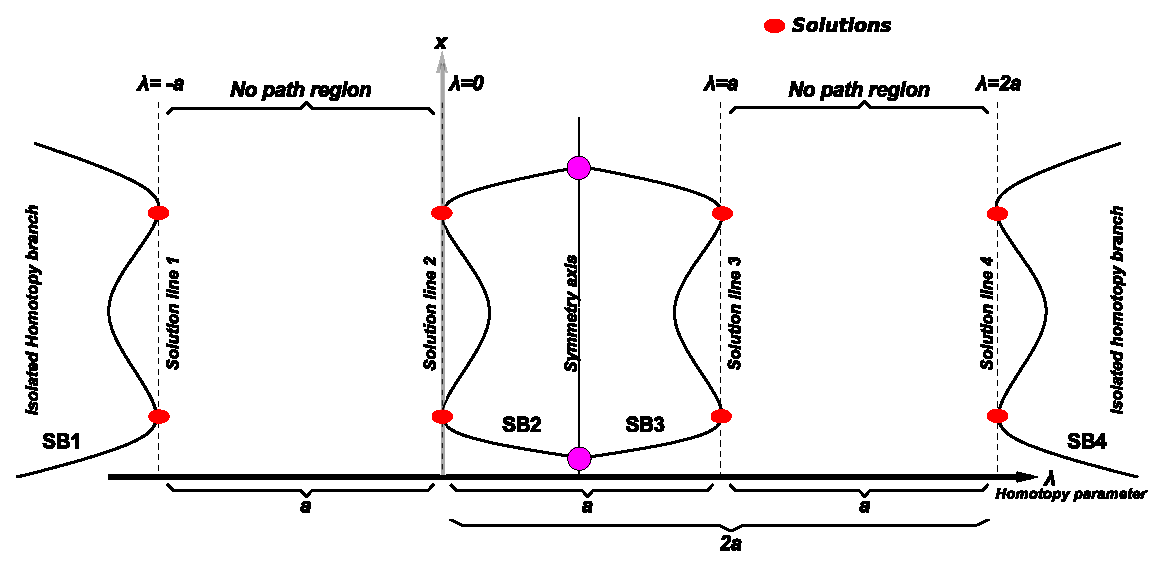
\includegraphics[scale=0.6]{yamamura/doblelineapoli.eps}}}
\caption{Double bounded homotopy with four solution lines.}
\label{doblehp}
\end{figure}

Fig. \ref{doblehp} shows how homotopy path starts at $A=(x_i,a/2)$ on the symmetry axis, finds two roots (in region $SB3$) and finishes when a new crossing through the symmetry axis at $B=(x_f,a/2)$ is detected, which means that tracing for a symmetrical branch has been completed and fulfilling the stop criterion \cite{homo_hk05}.


The properties for this new homotopy are presented in the following sub-sections:
\subsection{Symmetrical branches}

To obtain the branches for the homotopy path, first the equation \ref{homotopiaP} is reformulated as follows:

\begin{equation}
{%\tiny
\begin{array}{l}
H(f(x),\lambda )=\lambda(\lambda+a)(\lambda-a)(\lambda-2a)+(\lambda-a/2)^2 J(x)=0
\end{array}}
\label{homotopiaP1}
\end{equation}
where 
\begin{displaymath}
\begin{array}{l}
 J(x)= {Cf(x)^2 \over (x-x_i)(x-x_f)}
\end{array}
\end{displaymath}

In order to trace the homotopy path \cite{homo_hk05}, the unconnected symmetrical paths {\it SB1} and {\it SB4} will be ignored because these open branches would make not possible to apply the stop criterion. Symmetrical branches $SB2$ ($\lambda_2(x)$) and $SB3$ ($\lambda_3(x)$) shown in Fig. \ref{doblehp} can be derived solving $\lambda$ from equation \ref{homotopiaP1}. Given the fact that $SB2$ and $SB3$ are connected and symmetrical, only one should be traced to obtain the full path and finalize the simulation. $SB3$ is chosen as the tracing path, which tangentially touches the solution line $\lambda=a$. Therefore, the symmetrical branch $SB2$ is:

\begin{equation}
{%\tiny
\begin{array}{l}
\lambda_2(x)= {{a-\sqrt {5\,{a}^{2}-2\,\sqrt { \left( J \left( x \right) +4
\,{a}^{2} \right)  \left( J \left( x \right) +{a}^{2} \right) }+2\,J
 \left( x \right) }} \over {2}}
\end{array}}
\label{sb2}
\end{equation}


The symmetrical branch $SB3$ is:

\begin{equation}
{%\tiny
\begin{array}{l}
\lambda_3(x)= {{a+\sqrt {5\,{a}^{2}-2\,\sqrt { \left( J \left( x \right) +4
\,{a}^{2} \right)  \left( J \left( x \right) +{a}^{2} \right) }+2\,J
 \left( x \right) }} \over {2}}
\end{array}}
\label{sb3}
\end{equation}

To demonstrate that $\lambda_2(x)$ is linked to the solution line $\lambda=0$, the following limit is calculated:

\begin{equation}
 \displaystyle\lim_{f(x) \to{0}}{\lambda_2(x)}=0 
 \label{demos1x}
\end{equation}

the equilibrium equation $f(x)$ tends to zero when $x$ tends to solution $x^*$, as shown in the following limit calculation:

\begin{equation}
 \displaystyle\lim_{x \to{x^*}}{f(x)}=0 
 \label{demos1x2}
\end{equation}

Now, to demonstrate that $\lambda_3(x)$ is linked to the solution line $\lambda=a$, the following limit is calculated:

\begin{equation}
 \displaystyle\lim_{f(x) \to{0}}{\lambda_3(x)}=a 
 \label{demos2x}
\end{equation}

This shows that solutions $x^*$ are placed at $\lambda=a$.

\subsection{Symmetry axis}

The symmetry axis is an important property for the double bounded homotopy. In the particular case of the polynomial double bounded homotopy the symmetry axis is:

\begin{equation}
\lambda_{sym}= {a \over 2}
\label{sym}
\end{equation}

This symmetry axis belong to the symmetry relationship between $SB2$ and $SB3$ branches.

As shown in Fig. \ref{doblehp}, this relationship must be fulfilled:

\begin{displaymath}
\lambda_3(x)-\lambda_{sym}=\lambda_{sym} -\lambda_2(x)
\end{displaymath}

Replacing the value for $\lambda_{sym}$, we obtain:

\begin{displaymath}
\lambda_3(x)-0.5a=0.5a-\lambda_2(x)
\end{displaymath}

Then, replacing $\lambda_2(x)$ and $\lambda_3(x)$ for their respective functions the next relationship is found:

\begin{displaymath}
\begin{array}{l}
0.5a+0.5\sqrt{G(x)}-0.5a= 0.5a-0.5a+0.5\sqrt{G(x)}
\end{array}
\end{displaymath}

where {\small $G(x)=\sqrt {5\,{a}^{2}-2\,\sqrt { \left( J \left( x \right) +4 \,{a}^{2} \right)  \left( J \left( x \right) +{a}^{2} \right)}} $

Reducing terms:
\begin{displaymath}
\begin{array}{c}
0.5\sqrt{G(x)}=0.5\sqrt{G(x)} \\
0=0
\end{array}
\end{displaymath}

The proof for this equality shows that the homotopy path is symmetrical around the symmetry axis.

\section{Study case: circuit with bipolar transistors and a diode} 

In \cite{homo_yamamura}, a circuit was resolved using modified fixed point homotopy. This circuit has 3 operating points. The Ebers-Moll is used for all the transistors. The equation for the model is given as:

\begin{displaymath}
\left[ \begin{array}{c}
i_{D_E} \\
i_{D_C}
\end{array}\right] =
\left[ \begin{array}{cc} 1  & $-0.01$ \\
$-0.99$ & 1 \\
\end{array}\right] \left[ \begin{array}{c}
10^{-9}(e^{(40v_{be})} - 1) \\
10^{-9}(e^{(40v_{bc})} - 1)
\end{array}\right]
\end{displaymath}

As for the diode, the model is:

\begin{displaymath}
i_d=10^{-9}(e^{40u} - 1)
\end{displaymath}

First, the equilibrium equation is formulated using the modified nodal analysis with the result of a system having 14 equations ($f_1, f_2, \ldots, f_{14}$) and 14 variables ($v_1, v_2,\ldots,v_{13}, I_E$). The circuit is shown in Fig. \ref{yamaie}(a).



Now, double bounded homotopy is applied to solve the circuit; the homotopy formulation
is expressed as follows ($a=1, C=1$):

\begin{displaymath}
\begin{array}{c}
H_1(f_1,\lambda)=\lambda(\lambda+1)(\lambda-1)(\lambda-2)(v_1+13)(v_1-13)+(\lambda-0.5)^2 f_1^2=0\\
H_2(f_2,\lambda)=\lambda(\lambda+1)(\lambda-1)(\lambda-2)(v_2+13)(v_2-13)+(\lambda-0.5)^2 f_2^2=0\\
\vdots \\
H_{14}(f_{14},\lambda)=\lambda(\lambda+1)(\lambda-1)(\lambda-2)(I_E+13)(I_{E}-13)+(\lambda-0.5)^2 f_{14}^2=0\\
\end{array}
\end{displaymath}

The initial point for every electrical variable may take the value $+13$ or $-13$. Therefore, there are $n^2$ possible combinations for each initial point ($n$ is the number of electrical variables). In this simulation the initial point $x_i$ chosen is shown in Table \ref{yamamuracircuitosoluc}. The value $\pm 13$ is a safe way to include in the homotopy path all the operating points of the circuit to be analysed, which is biased with a voltage source ($E$) at 12V.

So, the next step is to solve the circuit using the double bounded homotopy, resulting in the convergence to the three known solutions for the circuit (Table \ref{yamamuracircuitosoluc}). The homotopy path correspondent to the nodal voltage $v_2$ is displayed in Fig. \ref{yamaie}(b) and Fig. \ref{yamaie}(c). Finally, the final point $x_f$ for the homotopy trace is exhibited in Table \ref{yamamuracircuitosoluc}. The appropriate selection of the initial point plays an important role on the number of solutions to be found, hereafter a study about an optimal initial point selection should be performed in a near future.


\section{Conclusion}
The stop criterion for homotopy methods consist in using a maximum number (arbitrarily number) of integration steps, in such a way that when integration steps reach the solution line the algorithm stops. Nevertheless, this kind of method may end without finding all roots on the homotopy path. A set of properties for the bounded homotopy were explained and developed. The bounded Homotopy with four solution lines shows interesting properties given by the fact that allows the homotopy path to be placed between two limits named solution lines. Also, the curvature radius on the solutions shows a proportional relationship with the separation between solution lines. Another fundamental property of this new homotopy is to possess a symmetry axis, which is found between solution lines ($\lambda=0$ and $\lambda=a$), allowing the implementation for a stop criterion. Finally, bounded homotopy with 4 solution lines was applied to DC simulation of a bipolar circuit example, showing its potential to be used on analysis of bipolar circuits.

\begin{table}[h]
{
\caption{Relevant points.}
\label{yamamuracircuitosoluc}
\small
\begin{center}
\begin{tabular*}{\textwidth}{@{\extracolsep{\fill}}||c|c|c|c|c|c|c|c|c||}
\hline\hline
R.P & $v_1$ & $v_2$ & $v_3$ & $v_4$ & $v_5$ & $v_6$ & $v_7$ & $v_8$\\ \hline
$x_i$ & +13 & -13 & +13 & -13 & -13 & -13 & -13 & -13\\ \hline
$S_1$ & 12 & 0.405 & 0.366 & 0.685 & 0.349 & 6.796 & 0.070 & 7.038 \\ \hline
$S_2$ & 12 & 0.883 & 0.278 & 0.590 & 0.631 & 0.812 & 0.315 & 1.074 \\ \hline
$S_3$ & 12 & 5.995 & 0.085 & 0.368 & 0.712 & 0.436 & 0.390 & 0.699 \\ \hline
$x_f$ & +13 & +13 & +13 & +13 & -13 & +13 & -13 & +13 \\ \hline
\end{tabular*}

\hspace{0.075in}

\begin{tabular*}{\textwidth}{@{\extracolsep{\fill}}||c|c|c|c|c|c|c|c||}
\hline
R.P cont. & $v_9$ & $v_{10}$& $v_{11}$ & $v_{12}$ & $v_{13}$ & $I_E$ & $ \lambda$\\ \hline
$x_i$ & -13 & -13 & -13 & -13 & -13 & -13 & 0.5  \\ \hline
$S_1$ & 11.839 & 0.4e-5 & 0.039 & 0.039 & 0.321 & -0.0085 & 1\\ \hline 
$S_2$ & 11.647 & 0.4e-5 & 0.039 & 0.039 & 0.321 & -0.0100 & 1 \\ \hline
$S_3$ & 11.635 & 0.4e-5 & 0.039 & 0.039 & 0.321 & -0.0089 & 1\\ \hline
$x_f$ & +13 & +13 & +13 & +13 & +13 & +13 & 0.5 \\ \hline
\hline
\end{tabular*}
\end{center}
}
\end{table}


\begin{figure*}[tbp]
\centering
\begin{minipage}{\linewidth}
\psfrag{r1}[Bl][bl][0.7]{$R_1=4k\Omega$}
\psfrag{r2}[Bl][bl][0.7]{$R_2=0.1k\Omega$}
\psfrag{r3}[Bc][bl][0.7]{$R_3=8k\Omega$}
\psfrag{r4}[Bc][bl][0.7]{$R_4=8k\Omega$}
\psfrag{r5}[Bl][bl][0.7]{$R_5=4k\Omega$}
\psfrag{r6}[Bl][bl][0.7]{$R_6=0.1k\Omega$}
\psfrag{r7}[Bc][bl][0.7]{$R_7=30k\Omega$}
\psfrag{r8}[Bl][bl][0.7]{$R_8=1k\Omega$}
\psfrag{r9}[Bl][bl][0.7]{$R_9=0.1\Omega$}
\psfrag{r10}[Bc][bl][0.7]{$R_{10}=10k\Omega$}
\psfrag{r11}[Bl][bl][0.7]{$R_{11}=4k\Omega$}
\psfrag{r12}[Bl][bl][0.7][-90]{$R_{12}=10k\Omega$}
\psfrag{r13}[Bl][bl][0.7][-90]{$R_{13}=1k\Omega$}
\psfrag{vcc}[Bl][bl][0.7]{$E=12V$}
\centering
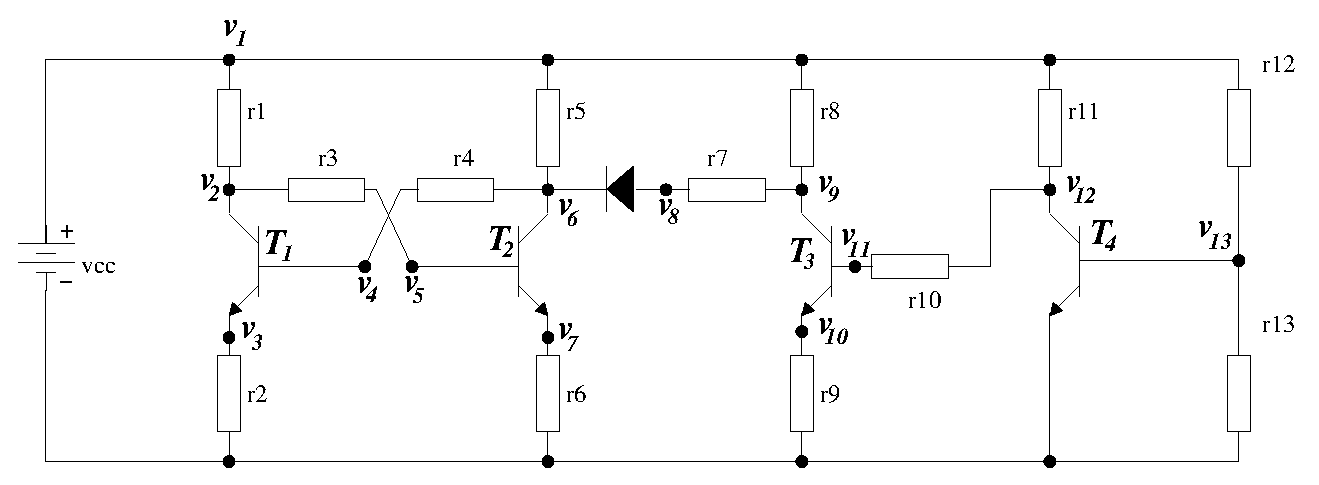
\includegraphics[scale=0.55]{yamamura/diotran.eps}
\end{minipage}
\newline
\begin{minipage}[l]{0.5\linewidth}
\centering
\begin{small}
\center (a)
\end{small}
\end{minipage}
\newline
\begin{minipage}[l]{0.5\linewidth}
	\centering
	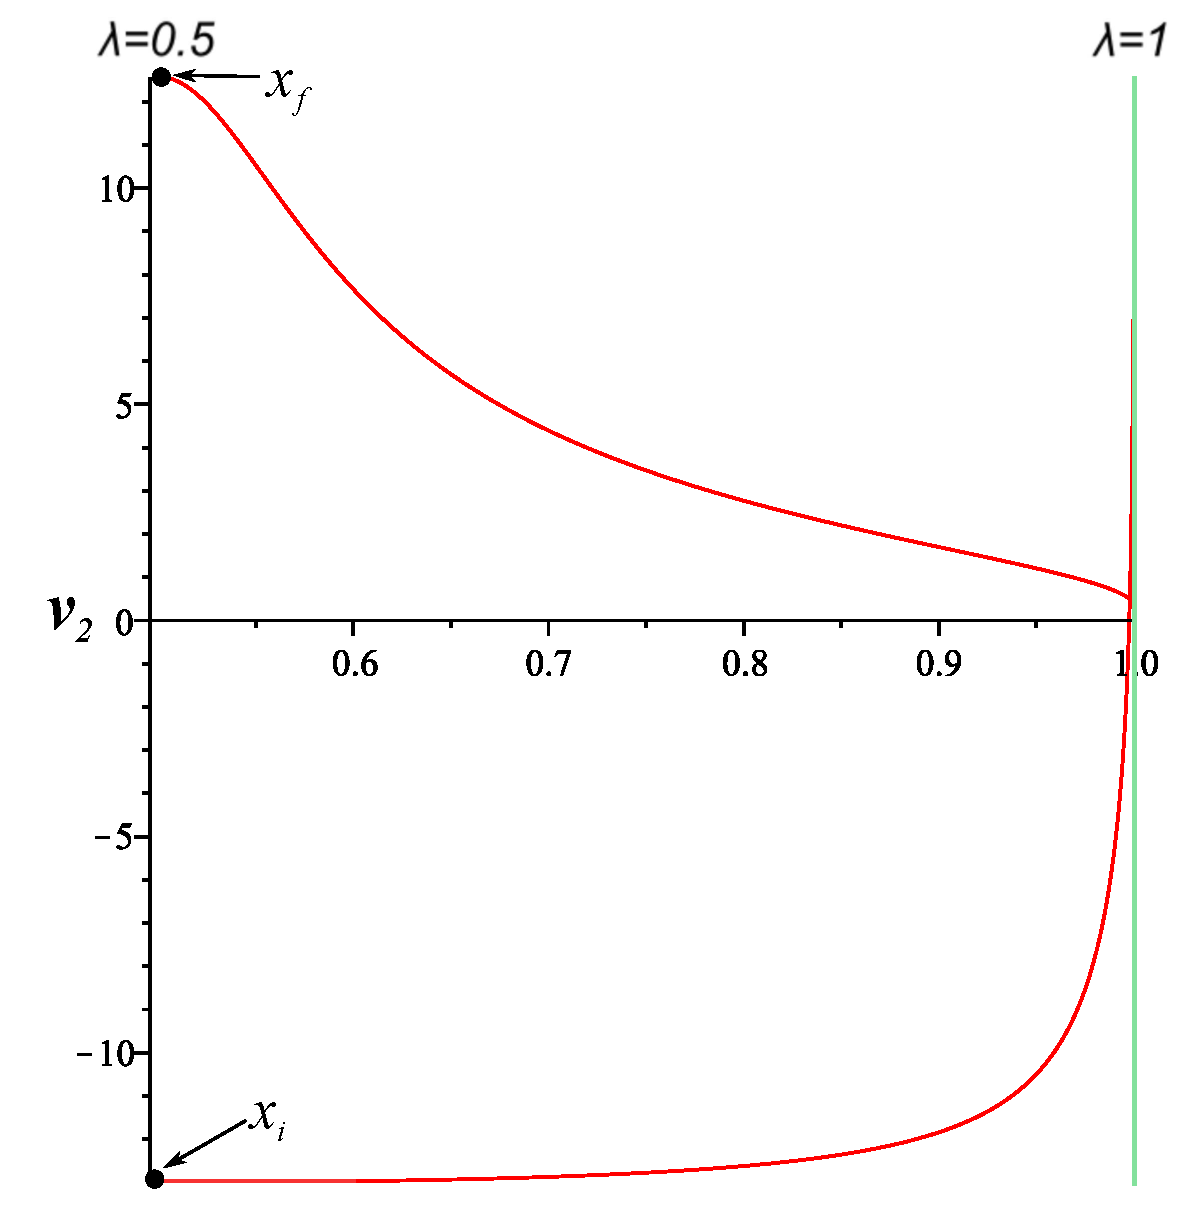
\includegraphics[scale=0.4]{yamamura/y1a.eps}
\end{minipage}
\newline
\begin{minipage}[l]{0.5\linewidth}
\centering
\begin{small}
(b)
\end{small}
\end{minipage}
\newline
\begin{minipage}[l]{0.5\linewidth}
	\centering
	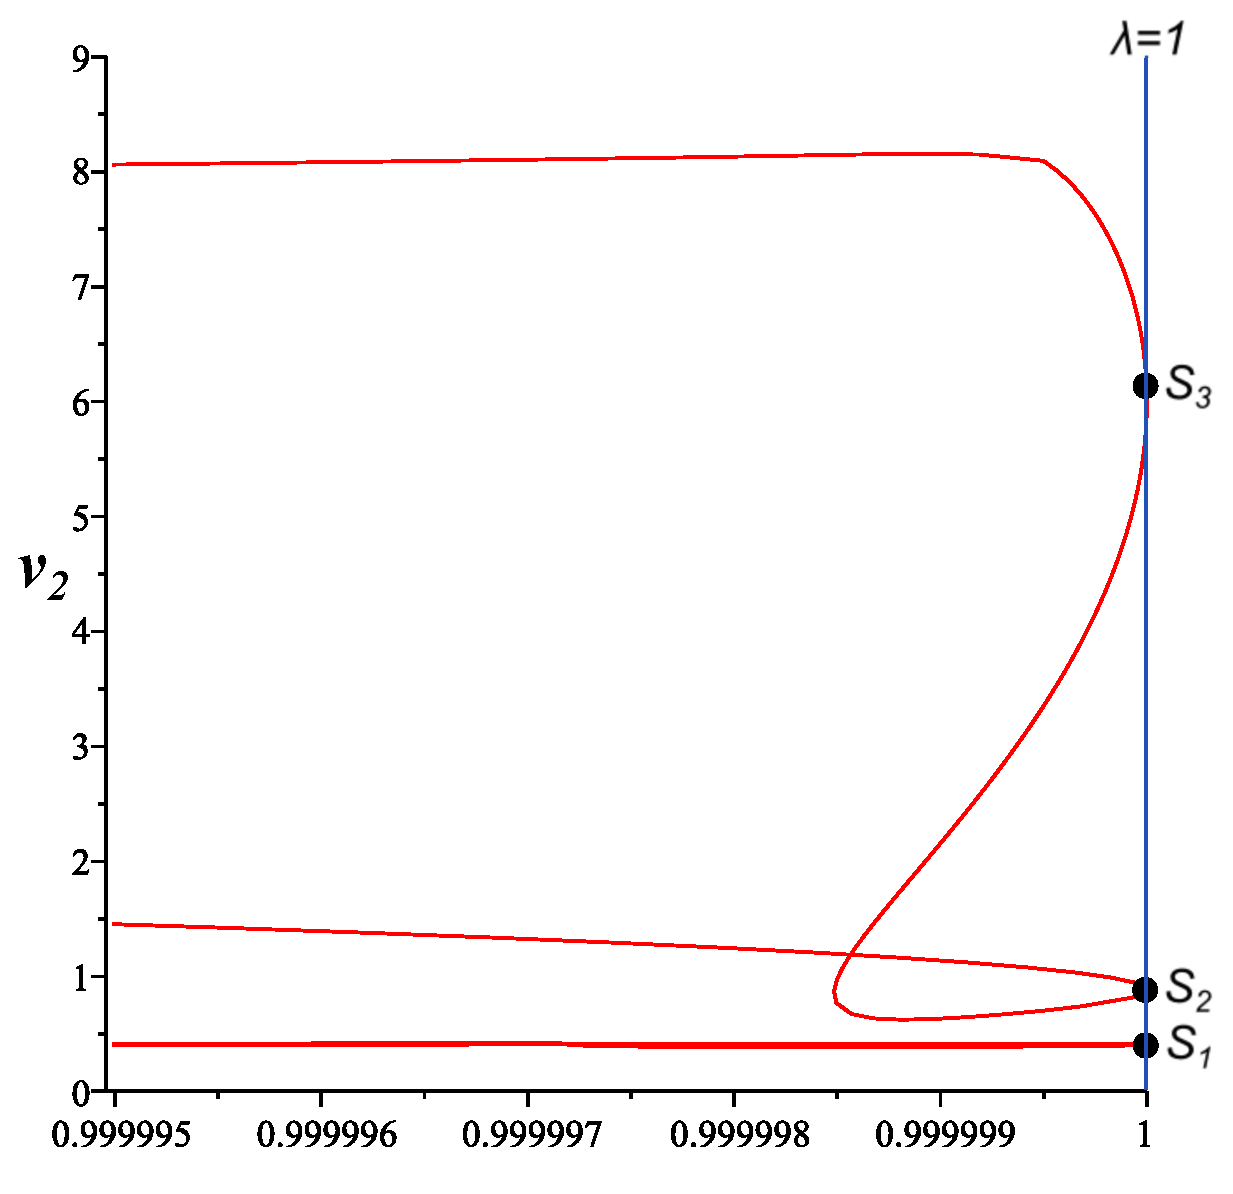
\includegraphics[scale=0.4]{yamamura/y1b.eps}
\end{minipage}
\newline
\begin{minipage}[l]{0.5\linewidth}
\centering
\begin{small}
(c)
\end{small}
\end{minipage}
\newline
\caption{(a) Benchmark circuit. (b) Homotopy path $\lambda-v_2$. (c) Zoom to the solution.}
\label{yamaie}
\end{figure*}


\end{document}
